\documentclass{standalone}

\usepackage{tikz}

\usetikzlibrary{calc}

\begin{document}
  %noformat{
  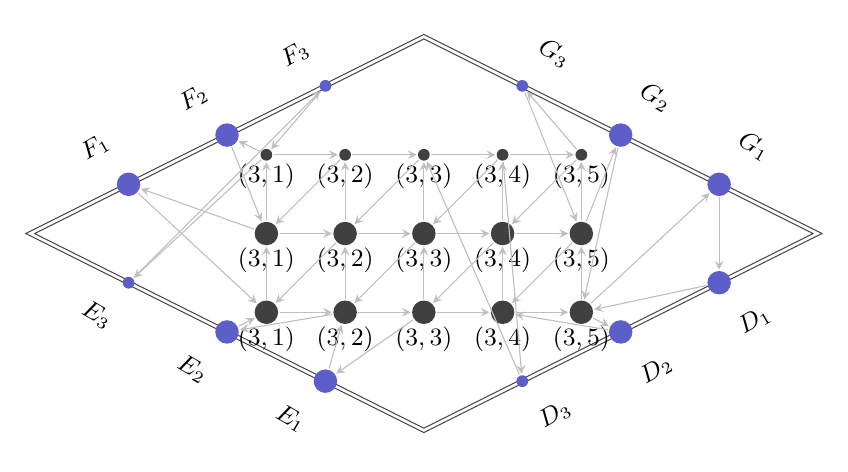
\begin{tikzpicture}
    \tikzset{font=\small}
    \tikzstyle{v1} = [circle, outer sep=0.5pt, fill, inner sep=1.5pt]
    \tikzstyle{v2} = [circle, outer sep=0.5pt, fill, inner sep=3.0pt]
    \tikzstyle{unf} = [color=darkgray]
    \tikzstyle{frz} = [color=blue!60!darkgray!70]
    \tikzstyle{e} = [color=lightgray, ->, >={stealth}]
    \tikzstyle{de} = [color=black, >={stealth}]
    \tikzstyle{b} = [fill, fill opacity=0.0, circle, outer sep=0.5pt, inner sep=1.5pt]
    \tikzstyle{te} = [color=darkgray, double distance=1pt]
    \tikzstyle{h} = [dashed, color=gray, ->, >={stealth}]
    \tikzstyle{ll} = [color=blue!60!darkgray!70]

    \coordinate (q_0) at (270:2.5);
    \coordinate (q_1) at (180:5.0);
    \coordinate (q_2) at ( 90:2.5);
    \coordinate (q_3) at (  0:5.0);

    \draw[te] (q_0) -- (q_1) -- (q_2) -- (q_3) -- cycle;

    \node[v2, frz, label={240:{\rotatebox{330}{$E_1$}}}   ] (E1) at ($ (q_0)!0.25!(q_1) $) {};
    \node[v2, frz, label={240:{\rotatebox{330}{$E_2$}}}   ] (E2) at ($ (q_0)!0.50!(q_1) $) {};
    \node[v1, frz, label={240:{\rotatebox{330}{$E_3$}}}   ] (E3) at ($ (q_0)!0.75!(q_1) $) {};

    \node[v2, frz, label={120:{\rotatebox{ 30}{$F_1$}}}   ] (F1) at ($ (q_1)!0.25!(q_2) $) {};
    \node[v2, frz, label={120:{\rotatebox{ 30}{$F_2$}}}   ] (F2) at ($ (q_1)!0.50!(q_2) $) {};
    \node[v1, frz, label={120:{\rotatebox{ 30}{$F_3$}}}   ] (F3) at ($ (q_1)!0.75!(q_2) $) {};

    \node[v2, frz, label={ 60:{\rotatebox{-30}{$G_1$}}}   ] (G1) at ($ (q_2)!0.75!(q_3) $) {};
    \node[v2, frz, label={ 60:{\rotatebox{-30}{$G_2$}}}   ] (G2) at ($ (q_2)!0.50!(q_3) $) {};
    \node[v1, frz, label={ 60:{\rotatebox{-30}{$G_3$}}}   ] (G3) at ($ (q_2)!0.25!(q_3) $) {};

    \node[v2, frz, label={-60:{\rotatebox{ 30}{$D_1$}}}   ] (D1) at ($ (q_0)!0.75!(q_3) $) {};
    \node[v2, frz, label={-60:{\rotatebox{ 30}{$D_2$}}}   ] (D2) at ($ (q_0)!0.50!(q_3) $) {};
    \node[v1, frz, label={-60:{\rotatebox{ 30}{$D_3$}}}   ] (D3) at ($ (q_0)!0.25!(q_3) $) {};

    \node[v2, unf, label={[label distance=-3pt]270:$(3,1)$}] (w15) at ($ (q_0)!0.30!(q_2) + (180:2.00) $) {};
    \node[v2, unf, label={[label distance=-3pt]270:$(3,1)$}] (w25) at ($ (q_0)!0.50!(q_2) + (180:2.00) $) {};
    \node[v1, unf, label={[label distance=-3pt]270:$(3,1)$}] (w35) at ($ (q_0)!0.70!(q_2) + (180:2.00) $) {};

    \node[v2, unf, label={[label distance=-3pt]270:$(3,2)$}] (w14) at ($ (q_0)!0.30!(q_2) + (180:1.00) $) {};
    \node[v2, unf, label={[label distance=-3pt]270:$(3,2)$}] (w24) at ($ (q_0)!0.50!(q_2) + (180:1.00) $) {};
    \node[v1, unf, label={[label distance=-3pt]270:$(3,2)$}] (w34) at ($ (q_0)!0.70!(q_2) + (180:1.00) $) {};

    \node[v2, unf, label={[label distance=-3pt]270:$(3,3)$}] (w13) at ($ (q_0)!0.30!(q_2)              $) {};
    \node[v2, unf, label={[label distance=-3pt]270:$(3,3)$}] (w23) at ($ (q_0)!0.50!(q_2)              $) {};
    \node[v1, unf, label={[label distance=-3pt]270:$(3,3)$}] (w33) at ($ (q_0)!0.70!(q_2)              $) {};

    \node[v2, unf, label={[label distance=-3pt]270:$(3,4)$}] (w12) at ($ (q_0)!0.30!(q_2) + (  0:1.00) $) {};
    \node[v2, unf, label={[label distance=-3pt]270:$(3,4)$}] (w22) at ($ (q_0)!0.50!(q_2) + (  0:1.00) $) {};
    \node[v1, unf, label={[label distance=-3pt]270:$(3,4)$}] (w32) at ($ (q_0)!0.70!(q_2) + (  0:1.00) $) {};

    \node[v2, unf, label={[label distance=-3pt]270:$(3,5)$}] (w11) at ($ (q_0)!0.30!(q_2) + (  0:2.00) $) {};
    \node[v2, unf, label={[label distance=-3pt]270:$(3,5)$}] (w21) at ($ (q_0)!0.50!(q_2) + (  0:2.00) $) {};
    \node[v1, unf, label={[label distance=-3pt]270:$(3,5)$}] (w31) at ($ (q_0)!0.70!(q_2) + (  0:2.00) $) {};

    \draw[e] (w13) -- (w12); \draw[e] (w12) -- (w11);
    \draw[e] (w23) -- (w22); \draw[e] (w22) -- (w21);
    \draw[e] (w33) -- (w32); \draw[e] (w32) -- (w31);

    \draw[e] (w15) -- (w14); \draw[e] (w14) -- (w13);
    \draw[e] (w25) -- (w24); \draw[e] (w24) -- (w23);
    \draw[e] (w35) -- (w34); \draw[e] (w34) -- (w33);

    \draw[e] (w15) -- (w25); \draw[e] (w25) -- (w35);
    \draw[e] (w14) -- (w24); \draw[e] (w24) -- (w34);
    \draw[e] (w13) -- (w23); \draw[e] (w23) -- (w33);
    \draw[e] (w12) -- (w22); \draw[e] (w22) -- (w32);
    \draw[e] (w11) -- (w21); \draw[e] (w21) -- (w31);

    \draw[e] (w34) -- (w25); \draw[e] (w33) -- (w24);
    \draw[e] (w24) -- (w15); \draw[e] (w23) -- (w14);

    \draw[e] (w31) -- (w22); \draw[e] (w32) -- (w23);
    \draw[e] (w21) -- (w12); \draw[e] (w22) -- (w13);

    \draw[e] (F3) -- (w35);
    \draw[e] (w35) -- (F2);
    \draw[e] (F2) -- (w25);
    \draw[e] (w25) -- (F1);
    \draw[e] (F1) -- (w15);

    \draw[e] (w13) -- (E1);
    \draw[e] (E1) -- (w14);
    \draw[e] (w14) -- (E2);
    \draw[e] (E2) -- (w15);
    \draw[e] (w35) -- (E3);
    \draw[e] (E3) -- (F3);

    \draw[e] (w31) -- (G3);
    \draw[e] (G3) -- (w21);
    \draw[e] (w21) -- (G2);
    \draw[e] (G2) -- (w11);
    \draw[e] (w11) -- (G1);

    \draw[e] (G1) -- (D1);
    \draw[e] (D1) -- (w11);
    \draw[e] (w11) -- (D2);
    \draw[e] (D2) -- (w12);
    \draw[e] (w32) -- (D3);
    \draw[e] (D3) -- (w33);

  \end{tikzpicture}
  %}noformat
\end{document}
